% Section content template for individual Educative lessons
% This file contains the actual content for a specific section
% Generated from Educative API section content

% Section: Design of Instagram
% Section ID: 5160831733465088
% Section Slug: design-of-instagram
% Generated: 2025-12-08T13:39:27.650019

\subsection{High-level design}\label{oW8g31uH3sRCfjfz9Yt4w}
\\
Our system should allow us to upload, view, and search images and videos at a high level. To upload images and videos, we need to store them, and upon fetching, we need to retrieve the data from the storage. Moreover , the users should also be allowed to follow each other.

\begin{figure}[htbp]
 \centering
 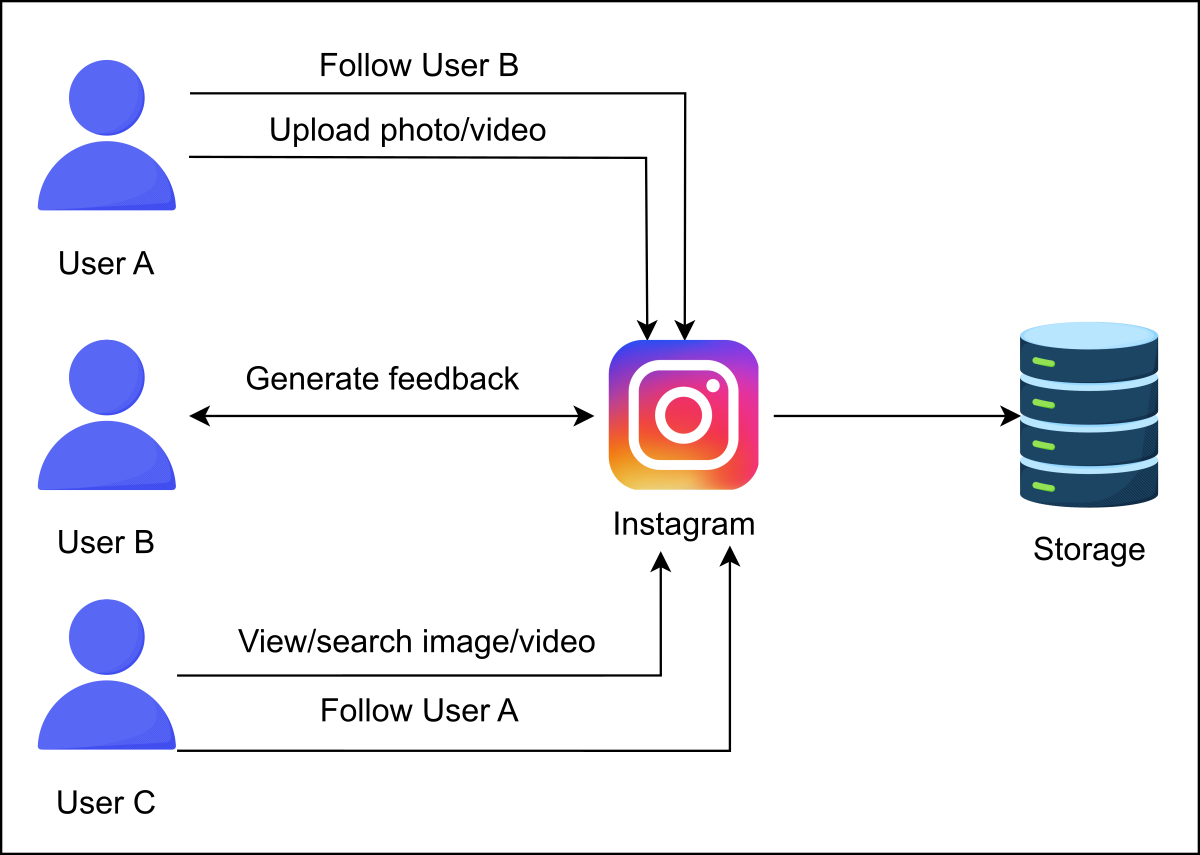
\includegraphics[width=0.5\textwidth]{Images/chapter_33/section_5160831733465088/5580167072579584.png}
 \caption{The high-level design of Instagram}
\end{figure}

\subsection{API design}\label{lytQC87J08qH-2hUtD6uA}
\\
This section describes APIs invoked by the users to perform different tasks (upload, like, and view photos/videos) on Instagram. We 'll implement REST APIs for these tasks. Let's develop APIs for each of the following features:

\begin{itemize}
\item
\protect\phantomsection\label{uNKYISATqtWdfLnFQRt6R}
Post photos and videos
\item
\protect\phantomsection\label{ZeZ5jRp3nmRv8xazodC5B}
Follow and unfollow users
\item
\protect\phantomsection\label{731szyN68mhJcOCLpt25S}
Like or dislike posts
\item
\protect\phantomsection\label{TYFlY-VFeCxnf-b-qWPXH}
Search photos and videos
\item
\protect\phantomsection\label{saWgm3adJCiEqiam4XFSA}
Generate a news feed
\end{itemize}
\\
All of the following calls will have a \texttt{userID}, that uniquely specifies the user performing the action. We 'll only discuss new parameters in the calls.

\subsubsection{Post photos or videos}\label{FgFC6KHHZt7yOm2fd0xDI}
\\
The POST method is used to post photos/videos to the server from the user through the \texttt{/postMedia} API. The
\texttt{/postMedia} API is as follows:

\begin{lstlisting}[language=JavaScript]
postMedia(userID, media_type, media_file, list_of_hashtags, caption)
\end{lstlisting}

\begin{table}[htbp]
\centering
\small
\adjustbox{max width=\textwidth}{
\begin{tabular}{|p{0.238\textwidth}|p{0.712\textwidth}|}
\hline
\textbf{Parameter} & \textbf{Description} \\
\hline
\hline
\texttt{media\_type} & It indicates the type of media (photo or video) in a post. \\
\hline
\texttt{media\_file} & It holds media file (photo or video) of a post. \\
\hline
\texttt{list\_of\_hashtags} & It represents all hashtags (maximum limit 30 hashtags) in a post. \\
\hline
\texttt{caption} & It is a text (maximum limit is 2,200 characters) in a user's post. \\
\hline
\end{tabular}
}
\end{table}

\subsubsection{Follow and unfollow users}\label{BBv7idRMNfUVDqoTfLtj9}
\\
The \texttt{/followUser} API is used when a user follows other users on Instagram. The \texttt{/followUser} API is as follows:

\begin{lstlisting}[language=JavaScript]
followUser(userID, target_userID)
\end{lstlisting}

\begin{table}[htbp]
\centering
\small
\adjustbox{max width=\textwidth}{
\begin{tabular}{|p{0.251\textwidth}|p{0.699\textwidth}|}
\hline
\textbf{Parameter} & \textbf{Description} \\
\hline
\hline
\texttt{target\_userID} & It indicates the user to be followed. \\
\hline
\end{tabular}
}
\end{table}

The \texttt{/unfollowUser} API uses the same parameters when a user unfollows someone on Instagram.

\subsubsection{Like or dislike posts}\label{HWvmHE0hlevk3ZruT2LlA}
\\
The \texttt{/likePost} API is used when users like someone's post on Instagram.

\begin{lstlisting}[language=JavaScript]
likePost(userID, post_id)
\end{lstlisting}

\begin{table}[htbp]
\centering
\small
\adjustbox{max width=\textwidth}{
\begin{tabular}{|p{0.251\textwidth}|p{0.699\textwidth}|}
\hline
\textbf{Parameter} & \textbf{Description} \\
\hline
\hline
\texttt{post\_id} & It specifies the post\textquotesingle s unique ID. \\
\hline
\end{tabular}
}
\end{table}

The \texttt{/dislikePost} API uses the same parameters when a user dislikes someone's post on Instagram.

\subsubsection{Search photos or videos}\label{QoYVkop5EwLWSs59Usoq2}
\\
The GET method is used when the user searches any photos or videos using a keyword or hashtag. The \texttt{/searchPhotos} API is as follows:

\begin{lstlisting}[language=JavaScript]
searchPhotos(userID, keyword)
\end{lstlisting}

\begin{table}[htbp]
\centering
\small
\adjustbox{max width=\textwidth}{
\begin{tabular}{|p{0.236\textwidth}|p{0.714\textwidth}|}
\hline
\textbf{Parameter} & \textbf{Description} \\
\hline
\hline
\texttt{keyword} \hfill\break & It indicates the string (username, hashtag, and places) typed by the user in the search bar. \\
\hline
\end{tabular}
}
\end{table}

\begin{quote}
\textbf{Note:} Instagram shows the posts with the highest reach (those with more likes and views) upon searching for a particular key. For example, if a user does a location-based search using ``London, United Kingdom," Instagram will show the posts in order with maximum to minimum reach. Instead of showing all the posts, the data will be loaded upon scrolling.
\end{quote}
\subsubsection{Generate news feed}\label{Vk5fD3v4xW0rBQaYKvbeG}
\\
The GET method is used when users view their news feed through the \texttt{/viewNewsfeed} API. The \texttt{/viewNewsfeed} API is as follows:

\begin{lstlisting}[language=JavaScript]
viewNewsfeed(userID, generate_timeline)
\end{lstlisting}

\begin{table}[htbp]
\centering
\small
\adjustbox{max width=\textwidth}{
\begin{tabular}{|p{0.236\textwidth}|p{0.714\textwidth}|}
\hline
\textbf{Parameter} & \textbf{Description} \\
\hline
\hline
\texttt{generate\_timeline} \hfill\break & It indicates the time when a user requests news feed generation. Instagram shows the posts that are not seen by the user between the last news feed request and the current news feed request. \\
\hline
\end{tabular}
}
\end{table}

Instagram introduced a new feature where users can filter the newsfeed generation request. Usually , the newsfeed is generated based on users\textquotesingle{} followers. But now there would be another option of favorite shows latest from the accounts chosen by the user.-\/-\textgreater{}

\subsection{Storage schema}\label{h8cZIiLphLBKUOVECXE8N}
\\
Let's define our data model now:

\subsubsection{Relational or non-relational database}\label{Jjg-NAnJ6Sd_zuxUwzN4M}
\\
It is essential to choose the right kind of database for our Instagram system, but which is the right choice---SQL or NoSQL? Our data is inherently relational, and we need an order for the data (posts should appear in chronological order) and no data loss even in case of failures (data durability). Moreover , in our case, we would benefit from relational queries like fetching the followers or images based on a user ID. Hence
, SQL-based databases fulfill these requirements.
\\
So, we'll opt for a relational database and store our relevant data in that database.

\subsubsection{Define tables}\label{OYzskl0mmUWV7DW_5CKc5}
\\
On a basic level, we need the following tables:

\begin{itemize}
\item
\protect\phantomsection\label{caKYqWqC2rIE4a0TUOuA7}
\textbf{Users}: This stores all user-related data such as ID, name, email, bio(An Instagram bio is a brief description of a user that appears beneath the username.), location, date of account creation, time of the last login, and so on.
\item
\protect\phantomsection\label{XvYf68hqcS2FE2cA1VaMG}
\textbf{Followers}: This stores the relations of users. In Instagram, we have a unidirectional relationship, for example, if user A accepts a follow request from user B, user B can view user A's post, but vice versa is not valid.
\item
\protect\phantomsection\label{gHt3Uvv72Rl2bxtpbmU3m}
\textbf{Photos}: This stores all photo-related information such as ID, location, caption, time of creation, and so on. We also need to keep the user ID to determine which photo belongs to which user. The user ID is a foreign key from the users table.
\item
\protect\phantomsection\label{naVW86wVaYKNhGfqbTEJy}
\textbf{Videos}: This stores all video-related information such as ID, location, caption, time of creation, and so on. We also need to keep the user ID to determine which video belongs to which user. The user ID is a foreign key from the users table.
\end{itemize}

\begin{quote}
\textbf{Quiz:}
\textbf{Question 1:} Where should we store the photos and videos?
\textbf{Answer:} We'll store the photos and videos in a blob store (like S3) and save the path of the photo or video in the table as it is efficient to save larger data in a distributed storage.
\end{quote}

The following illustration visualizes the data model:

\begin{figure}[htbp]
 \centering
 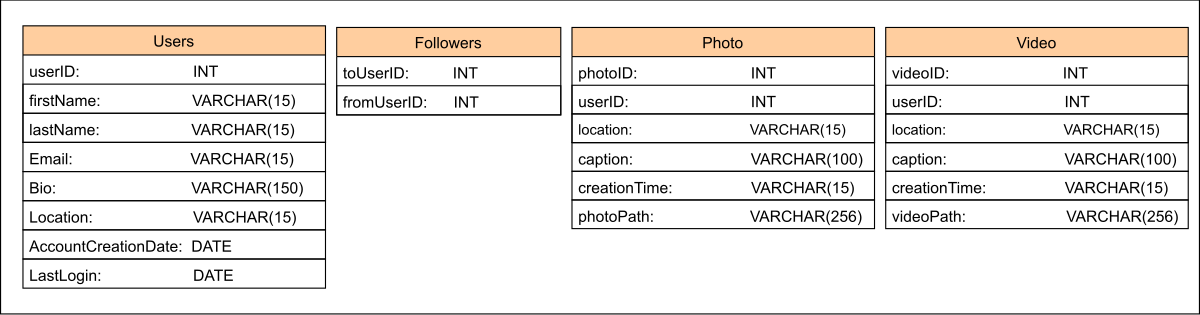
\includegraphics[width=0.5\textwidth]{Images/chapter_33/section_5160831733465088/6668712279277568.png}
 \caption{The Data model of Instagram}
\end{figure}

\subsubsection{Data estimation}\label{KuEHL9O4TJnzjPM2yy-oM}
\\
Let's figure out how much data each table will store. The column per row size (in bytes) in the following calculator shows the data per row of each table. It also calculates the storage needed for the specified counts. For example, the storage required for 500 million users is 111000 MB, 2000 MB for 250 followers of a single user, 23640 MB for 60 million photos, and 13790 MB for 35 million videos.
\\
You can change the values in the calculator to observe the change in storage needed. This gives us an estimate of how fast data will increase in our tables.

\begin{quote}
\textbf{Note:} Most modern services use both SQL and NoSQL stores. Instagram officially uses a combination of SQL (PostgreSQL) and No-SQL (Cassandra) databases. The loosely structured data like timeline generation is usually stored in No-SQL, while relational data is saved in SQL-based storage.
\end{quote}
\\
In the next lesson, we'll identify more components to tweak our design.

% End of section content